%
\documentclass[12pt,a4paper]{article}

\usepackage[utf8]{inputenc}
\usepackage[usenames,dvipsnames]{xcolor}
\usepackage{graphicx}
\usepackage[margin=1in]{geometry}
\usepackage[]{natbib}
\usepackage[]{sidecap}
\usepackage{setspace}
\usepackage{defs}
\usepackage{lastpage}
\usepackage{fancyhdr}
\usepackage{pdfpages}
\usepackage{enumitem}

\usepackage{libertine}
\usepackage[T1]{fontenc}

\usepackage[pdftex]{hyperref}
\hypersetup {
    bookmarks=true,                    % show bookmarks bar in pdf reader
    pdftitle={Research Proposal - 2016 VR Etableringsbidrag},                   
    pdfauthor={Gregory A. Feiden},     % set pdf author
    pdfsubject={}, % pdf subject
    colorlinks=true,                   % false = box link, true = colored links
    linkcolor=black,                   % color of internal links
    citecolor=black,                    % color of citations
    urlcolor=NavyBlue                      % external url color
}
\urlstyle{same}

\citestyle{aa}
\bibliographystyle{mn}

\pagestyle{fancy}
\fancyhead[L]{Gregory Feiden -- Personal Number -- Research Plan}
\fancyhead[R]{\thepage\ of\ \pageref{LastPage}}
\fancyfoot[C]{}
\renewcommand{\headrulewidth}{0.0pt}

\fancypagestyle{plain}{
    \fancyhf{}
    \fancyfoot[C]{\thepage\ of\ \pageref{LastPage}}
    \renewcommand{\headrulewidth}{0.0pt}
    \renewcommand{\footrulewidth}{0.0pt}
}

\setlength{\parindent}{0pt}
\setlength{\parskip}{0.5\baselineskip}
\newenvironment{myindentpar}[1]%
 {\begin{list}{}%
         {\setlength{\leftmargin}{#1}}%
         \item[]%
 }
 {\end{list}}

\begin{document}

\begin{center}
	{\bf {\LARGE Ages of Young Stars and the Evolution 
	
	of Dynamo-Generated Magnetic Fields}} 
\end{center}

Astrophysical phenomena generally occur over time periods inaccessible to even the most patient human. Typical timescales range from thousands to billions of years. Nevertheless, time dependence is a vital component in our understanding astrophysical processes. 
%To overcome the difficulties 
Instead of monitoring a single system over time, astronomers gain insight into the time dependence of astrophysical phenomena by considering an ensemble of systems at different ages. Individual systems provide snapshots in time and a chronological ordering produces a stop-motion film of various processes across cosmic time. Accurate absolute ages are therefore the most sought after astrophysical quantities. This is particularly true for young systems, where ages provide critical constraints on the formation of stars, planets, and objects in-between. However, despite their importance, accurate ages for young systems remain elusive.

\vspace{\baselineskip}

{\bf \large Purpose and Aims}

\clearpage

{\bf \large Survey of the Field}
\begin{itemize}
	\item Age-dating problems for young stars. (i.e., model inconsistencies)
	\item Identification / inclusion of magnetic fields in models. (D'Antona, MacDonald, Feiden)
	\item Magnetic field observations. (e.g., MDI, ZDI)
	\item Open questions.
\end{itemize}

\begin{figure}
	\centering
	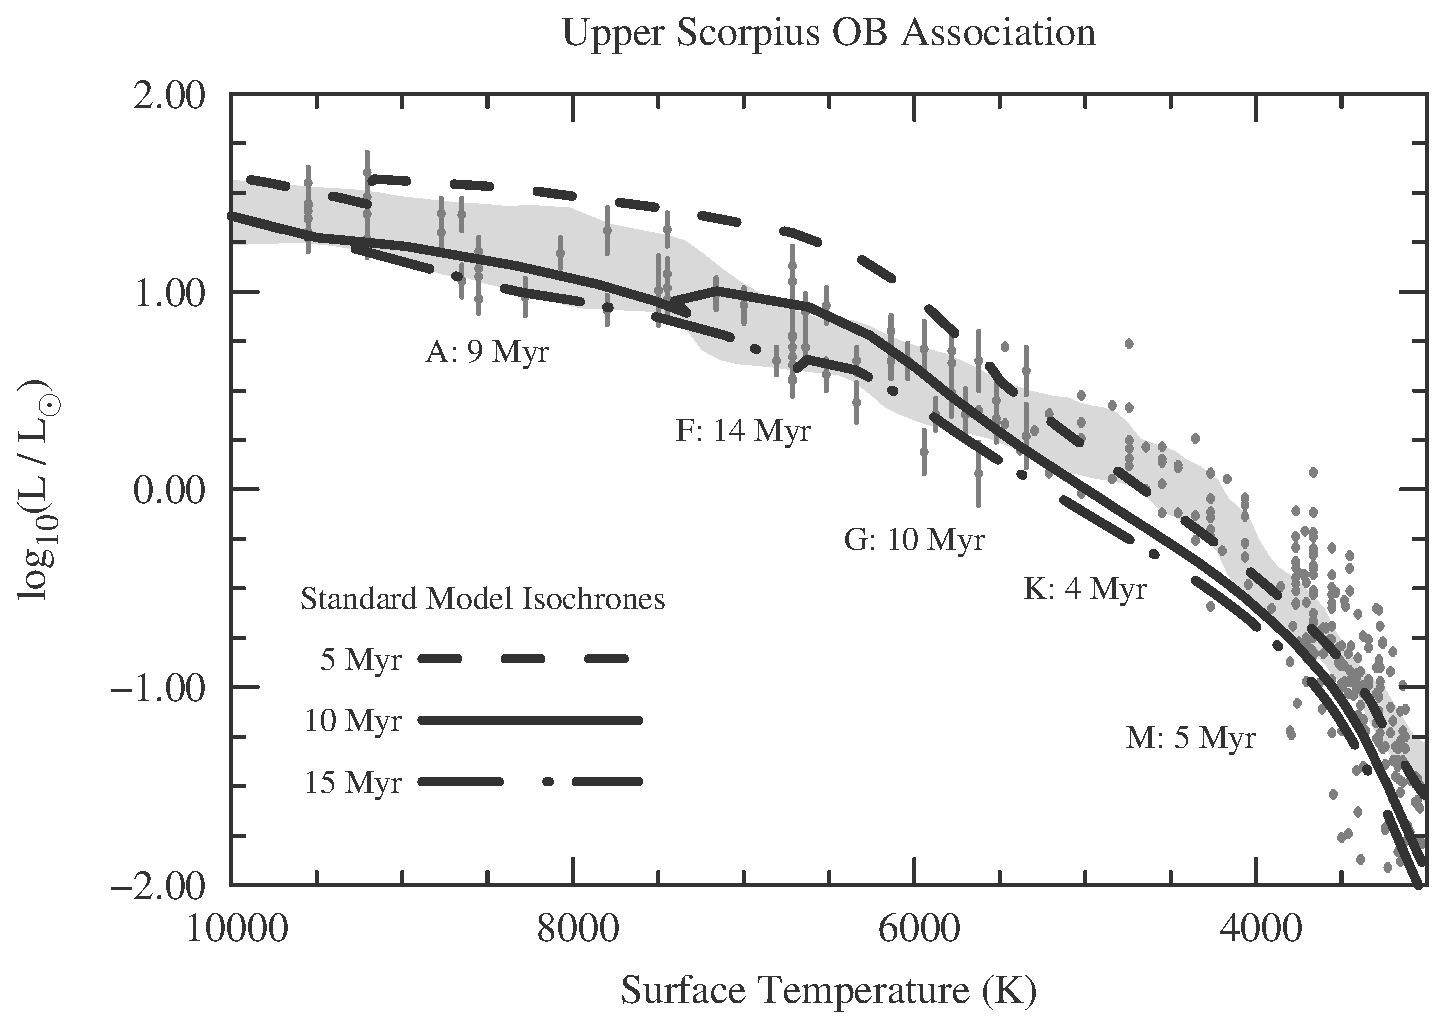
\includegraphics[width=0.75\linewidth]{./fig/USco_Age_Problems.eps}
	\caption{Caption.}
	\label{fig:probs}
\end{figure}

\begin{figure}
	\centering
	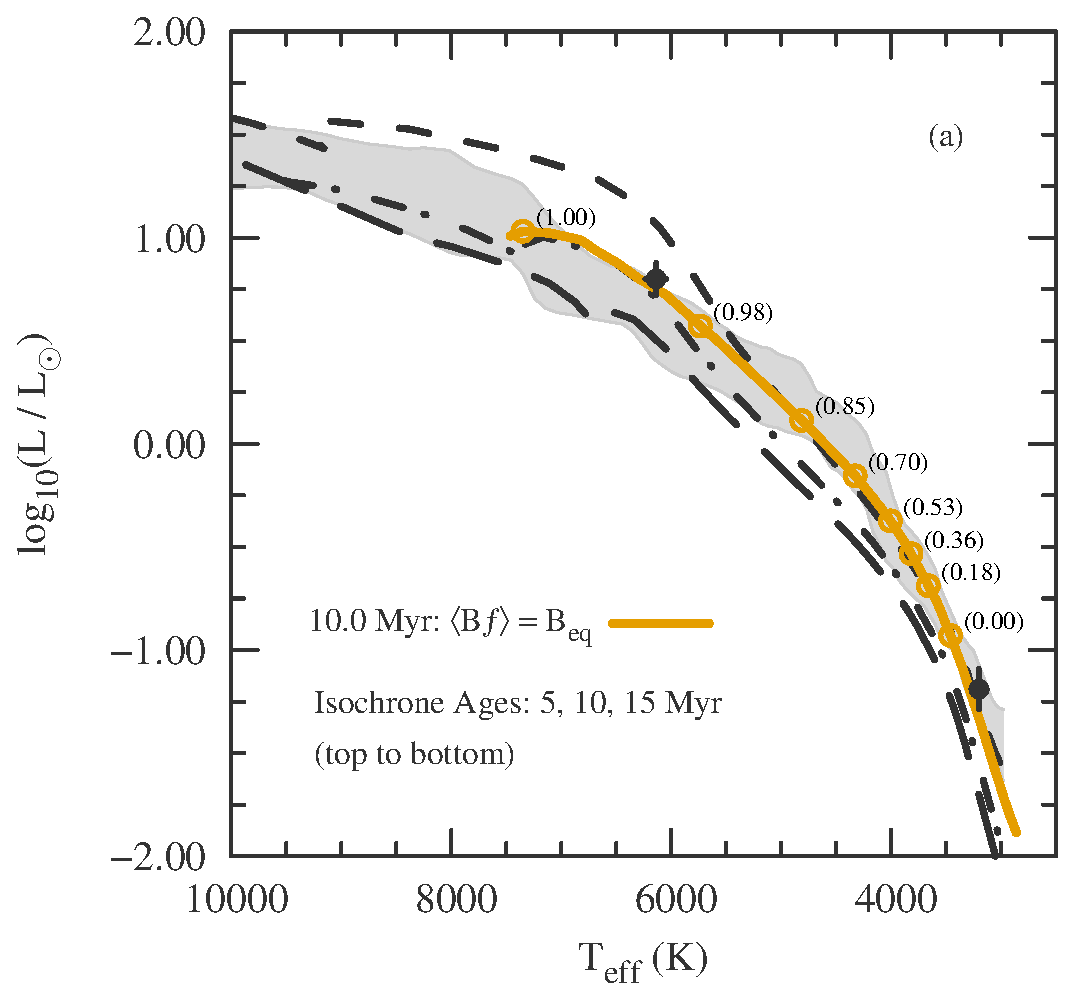
\includegraphics[width=0.45\linewidth]{./fig/USco_HR_diagram.eps} \qquad
	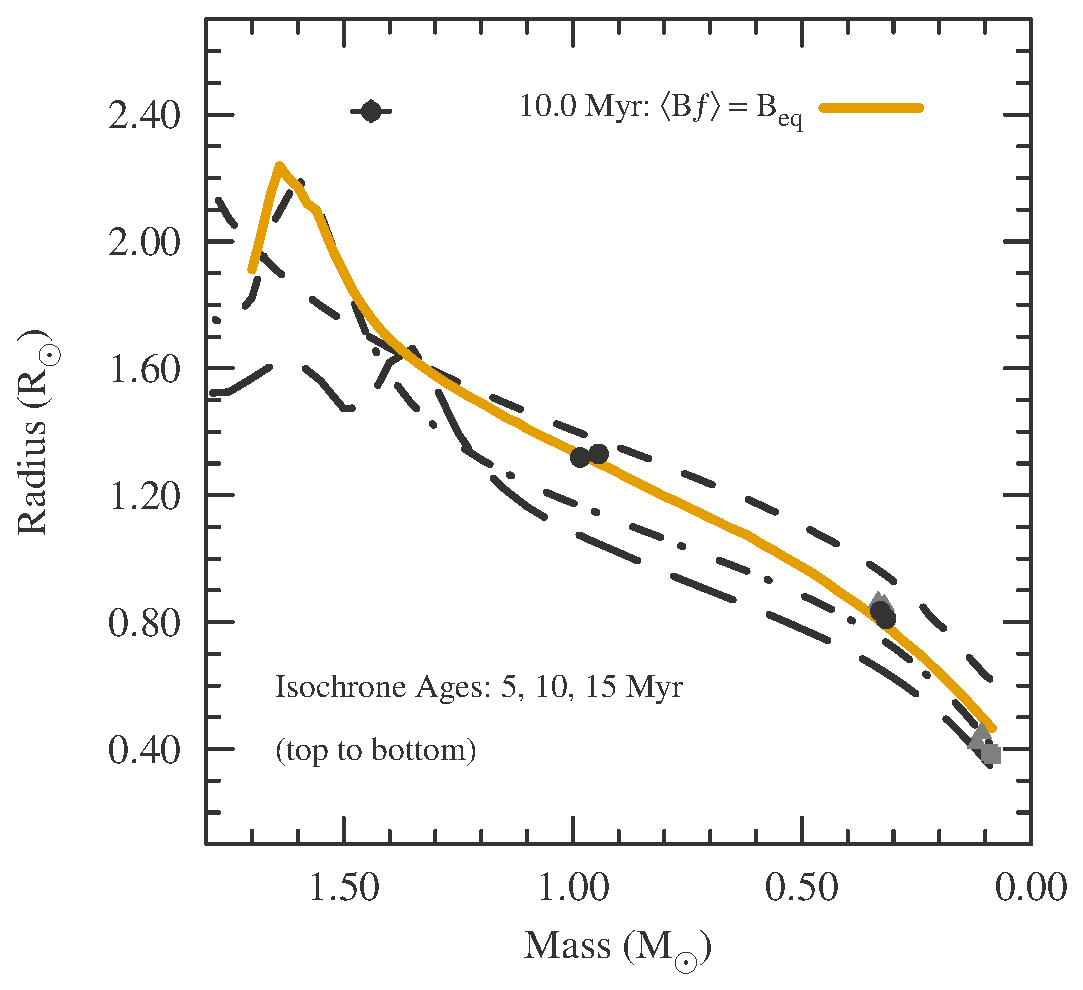
\includegraphics[width=0.45\linewidth]{./fig/USco_MR_diagram.eps}
	\caption{Caption.}
	\label{fig:usco}
\end{figure}

{\bf \large Project Description}

\textbf{P1. Dynamo-Generated Magnetic Fields throughout Stellar Evolution} \\
Describe coupling of stellar evolution and mean-field dynamo theory. 

This project is subdivided into three sub-projects denoted SP1, SP2, and SP3. Each sub-project focuses on a particular stage of stellar evolution from the pre-main-sequence through the first ascent red giant branch. The majority of the project's focus will be on SP1: the early evolution of dynamo generated magnetic fields. Although relatively brief compared to full evolutionary timescales, pre-main-sequence evolution dictates... and has far reaching implications for... Continuing evolution beyond the pre-MS comes at a very small computational cost. Evolution along the main-sequence can be modeled with very little computational time. Recently, magnetic fields have been proposed to explain several observational phenomena revealed by the \kepler\ Space Telescope \citep{Fuller2015, vanSaders2016}. The code we propose to develop provides an opportunity to study the physics underlying the observed phenomena. Therefore, we will allow stars and their dynamo-generated magnetic fields to evolve along the main-sequence and up the red giant branch. 
%By doing so, we will be able to explore several open questions in stellar evolution in which magnetic fields have been implicated.

\textbf{\textit{SP1. Pre-Main-Sequence Evolution}} \\
Magnetic inhibition of convection, magnetic field topology, rotational evolution, activity cycles.

\textbf{\textit{SP2. Main-Sequence Evolution}} \\
Rotational evolution, wind breaking, magnetic field topology, dynamo shifts at the fully convective boundary, activity cycles.

\textbf{\textit{SP3. Post-Main-Sequence Evolution}} \\
Depletion of hydrogen in stellar cores eventually reaches a level... Stars begin to traverse across the HR diagram along the sub-giant branch and up the first-ascent red giant branch once hydrogen shell burning ceases. Stars more massive than approximately 1.2 Msun possess a convective core along the hydrogen burning main sequence that is able to sustain a dynamo-generated magnetic field \citep[e.g.,][]{Browning2004,Featherstone2009,Augustson2016}. Upon leaving the main sequence, however, convection in the stellar core rapidly subsides (8 Myr). The fate of the dynamo-generated magnetic fields produced by the convective core during this period of rapid transition off the main-sequence is unexplored. 

There is indirect evidence from asteroseismology that remnant magnetic fields exist in the convectively stable cores of in a fraction of red giant branch stars. Most red giant branch stars observed by Kepler pulsate at specific frequencies that are characteristic of a coupling between wave-modes generated in the radiative stable core and modes created in convectively unstable outer envelope. However, a fraction of stars in the Kepler exhibit a very weak, if not non-existent, coupling between these wave modes \citep{Fuller2015}. The current hypothesis is that strong magnetic fields left over from the dynamo-generation process inhibit the propagation of g-modes in the radiative core, a so-called ``magnetic greenhouse effect,'' ultimately suppressing the coupling of modes between the core and envelope \citep{Fuller2015, Cantiello2016}. However, it is unclear whether rapidly shrinking convective cores are able to produce remnant magnetic fields that are strong enough (strength) or posses a proper topology (predominantly dipolar?) to efficiently suppress mode coupling. 
% coupling to radiative zone as convective core recedes?

{\it We will study how the strength and topology of dynamo-generated magnetic fields evolve in the cores of intermediate-mass stars leading up to, during, and following their transition off the main sequence.} Detailed magnetohydrodynamic simulations show that convective cores can sustain magnetic dynamos and that the resulting magnetic field can affect the properties of convection.


\textbf{P2. \emph{Dynamo-Generated Magnetic Fields in Brown Dwarfs and Giant Planets}} \\
Delayed contraction in stars. What about in brown dwarfs and giant planets? Affect their thermal history and thus masses that we infer for directly imaged objects. Impacts formation theories (via mass distribution) and even the status of an object (star vs bd, bd vs planet).

\textbf{P3. \emph{Fundamental Properties of Young Single Stars}} \\
Inferring accurate ages for young stars requires that stellar evolution models predict accurate fundamental properties for real stars. {\it This project focuses on confronting model predictions of young star properties as a function of age using a large number of well-characterized stars and young eclipsing binaries observed by Kepler/K2.}
Previous investigations have found that young stellar models are unable to accurately predict effective temperatures and luminosities for stars at a given mass \citep[e.g.,][]{Hillenbrand2004, Mathieu2007, Stassun2014}. These studies have focused on astrometric and eclipsing binaries (EBs), making it difficult to rule out whether binarity is playing a role in driving disagreements. Even wide binaries may be subject to subtle interactions that corrupt agreement with models. Recently, \citet{Stassun2014} showed that, while binarity in and of itself may not be a problem, model errors appear to be correlated with the presence of a tertiary companion. Triplicity among the sample of eclipsing binaries in \citet{Stassun2014} was well above 50\%, reducing the sample of potentially reliable comparisons to models. Our understanding about whether young stellar models are accurate at predicting properties of single stars may therefore be biased.

{\it Therefore, we are creating the first large sample of single young benchmark stars, whose fundamental properties will be measured with high precision} (better than 5\% for young stars). Stellar properties are derived using flux-calibrated spectra obtained by collaborators Mann and Gaidos. The spectra are used to derive bolometric fluxes and effective temperatures, leading to empirical estimates of stellar radii. This technique was proven to be robust for assessing stellar evolution model reliability for main sequence field stars \citep{Mann2015b}. Our current target sample contains 130 young stars in nearby moving groups and young stellar associations with known distances.

Comparison of properties of benchmark stars to stellar models will be performed using Bayesian inference to derive best fit model properties with realistic uncertainties \citep{Mann2015b}. We will then explore how well models reproduce the observed data and whether there are any noticeable correlations with additional observables, such as magnetic activity indicators, inferred age, chemical composition, and the convective mixing length parameter. Since we are targeting stars that are members of known young moving groups and associations, we will check that models yield consistent ages and distances to stars from a common group. If there are inconsistencies, we will attempt to characterize them in terms of observables and inferred stellar model parameters.

\textbf{P4. \emph{Homogeneous Ages for Young Stellar Associations}} \\
Deriving homogeneous ages for young stellar associations using available literature data. Provides constraints on a number of interesting astrophysical phenomena. [partially with UT Austin; Stockholm]

Informed by results obtained in projects 1, 2, and 3, we will bring together all of the information to establish ages for young stellar systems that are consistent for different age measures. The age determinations will fold in all necessary ingredients, starting with a base set of standard young stellar models and exploring whether magnetic fields, starspots, or chemical composition are able to provide complete agreement for each system. We?ll explore the possibility that the appropriate mix of ingredients from work package 1 and other modified physics from work package 2 lead to consistent ages for all systems or if there are correlations among the mix of ingredients and stellar system parameters like age.

To avoid being entirely dependent on the success of WP01 and WP02, we will begin an initial effort characterizing how magnetic stellar models developed by GAF perform in terms of predicting consistent ages given different age indictors. Notably, consistency between high- and low-mass regions of CMDs and the HRD, as well as the lithium depletion boundary. We have preliminary results using a single eclipsing binary in Upper Sco (Kraus et al. 2015) that indicates magnetic models may provide favorable consistency between different mass regimes and between different age indicators for the binary alone (see Figure 2). We will therefore try to develop a more complete analysis of Upper Sco, including more archival data, and other nearby YMGs to determine the robustness of the solution. We will also provide our magnetic models to the community to permit additional independent efforts to evaluate the success or failures of these models.

Results of this exercise will be important, whether or not we are able to derive consistent ages or the different stellar systems. If we can derive consistent ages, then that will provide strong support for those derived ages, at least for the moment, which will become a powerful resource for the astronomical community. If we cannot, then we learn that there is yet something missing from models or that our initial hypothesis that low-mass stars are to blame for the systematic age differences observed in young stellar systems is incorrect.


Finally, this sub-project requires production of a grid of pre-main-sequence magnetic stellar models. Since the grid will be produced concurrently with the above studies, no additional time will be required. Local clusters at Uppsala will provide computational resources necessary and the PI is applying for time with SNIC, the Swedish high-performance computing center. All models, data products, and analysis tools will be made publicly available.

\clearpage

{\bf \large Significance}
\begin{itemize}
  \item Ages of Young Stars
  	\begin{itemize}
    	\item protoplanetary disk evolution timescales
    	\item giant planet formation timescales
    	\item star formation history, including time dependence of IMF
    	\item properties of directly imaged planets and brown dwarfs (mass distribution --> formation)
  	\end{itemize}
  \item Magnetic Field Evolution
  	\begin{itemize}
    	\item activity cycles --> astrobiology (stretch?)
    	\item angular momentum transport and stellar rotational evolution
    	\item accurate stellar properties
		\begin{itemize}
      		\item ages and masses of single stars
      		\item properties of transiting extrasolar planets
		\end{itemize}
     \end{itemize}
  \item Grid of Stellar Models
  	\begin{itemize}
		\item available to public
    	\item allows extensive testing of theory
	\end{itemize}
  \item Relevance for Next-Generation Surveys
\end{itemize}

{\bf \large Preliminary Results} \\
Feiden (2016, submitted). Identification of magnetic fields as culprit for age discrepancies.

Pilot study for the Sun (and low-mass star?).

Feiden \& Christophe (in preparation). Parametrized model of starspots.

Stars characterized for CALYPSO thus far.

{\bf \large Independent Line of Research}
\begin{itemize}
	\item Calibration of Low-Mass Young Stars and their Planetary Systems with Observations (CALYPSO): 
	second avenue of research is characterizing planets around young stars. 
    Feiden (projectledare) provides a comprehensive analysis of host stars using stellar models coupled 
    with Bayesian inference
    to give stellar mass, age, and distance estimates with realistic uncertainties.
	\item 4MOST Internal Working Group 7 -- Galactic Analysis Pipeline -- providing stellar
    structure and atmosphere code for self-consistent determination of atmospheric 
    parameters, mass, and ages for over 1 million stars.
    \item Zodiacal Exoplanets in Time (ZEIT).
\end{itemize}

{\bf \large International and National Collaborations}
\begin{itemize}
  	\item [Confirmed] Star formation group at UT Austin (Kraus, Rizzuto). Fundamental properties of young stars using B- through M-type EBs in young associations with Kepler/K2. Magnetic fields of young stars with IGRINS.
  	\item [Confirmed] CALYPSO: Calibration of Low-mass Young stars and their Planetary Systems with Observations (Mann [UT Austin], Gaidos [Hawaii], Ansdell [Hawaii]). Fundamental properties of bona fid\'{e} members of nearby young moving groups using "spectro-bolometric techniques."
  	\item [Pending] MDI/ZDI research group at ESO (Hussain, Lavail). Magnetic field topologies for young T-Tauri stars that can be compared against predictions from models in P1 with age information from P3.
  	\item [Pending] MDI/ZDI research group at Uppsala (Kochukhov, Ros\'{e}n). Magnetic field topologies for young solar analogs in young stellar associations.
  	\item [Confirmed] Open Cluster collaboration (Silvester, Landstreet). Magnetic field topologies for intermediate mass stars in several young stellar associations.
\end{itemize}


{\bf \large Other Grants}

\bibliography{/Users/grefe950/Dropbox/papers}

\end{document}
